\documentclass[10pt,conference,letterpaper]{IEEEtran} 

\usepackage{url}
\usepackage[noadjust]{cite}
\usepackage[font=small]{caption}
\usepackage{subcaption}

\usepackage{xcolor}
\usepackage[pdftex]{graphicx}
\graphicspath{{../media/}}
\DeclareGraphicsExtensions{.pdf,.jpeg,.png}

\usepackage[cmex10]{amsmath}
\usepackage{amssymb}
\usepackage{mathtools}
\usepackage{amsthm}
\newtheorem*{theorem*}{Theorem}
\renewcommand{\IEEEQED}{\IEEEQEDopen}

\usepackage{algorithm}
\usepackage[noend]{algpseudocode}
\algnewcommand\Payload{\textbf{payload} }
\algnewcommand\Update{\textbf{update} }
\algnewcommand\Query{\textbf{query} }
\algnewcommand\Compare{\textbf{compare} }
\algnewcommand\Merge{\textbf{merge} }
\algnewcommand\Pre{\textbf{pre} }
\algnewcommand\Let{\textbf{let} }
\algnewcommand\Prepare{\textbf{prepare}}
\algnewcommand\Effect{\textbf{effect}}

\usepackage{setspace}

\begin{document}

\title{A Scalable Conflict-free Replicated Set Data Type}

\author{
\IEEEauthorblockN{Andrei Deftu}
\IEEEauthorblockA{1\&1 Internet AG\\andreideftu@gmail.com}
\and
\IEEEauthorblockN{Jan Griebsch}
\IEEEauthorblockA{1\&1 Internet AG\\jan.griebsch@1und1.de}
}

\maketitle

\begin{abstract}
Data replication is the fundamental approach to achieve load balancing,
scalability, and fault tolerance. In order to maintain replicas of some mutable
shared object consistent, synchronization is usually needed.
\textit{Conflict-free Replicated Data Types} (CRDTs) ensure eventual
consistency, such that replicas converge to a common state, equivalent to a
correct sequential execution without foreground synchronization.

A particular CRDT is the \textit{set} data type, for storing a collection of unique
elements. We improve this type specification by introducing an efficient
algorithm for sending deltas of updates between replicas and by partitioning a
set replica into disjunctive subsets. We add support for limited-lifetime
elements and solve the problem of unbounded database growth through a garbage
collection mechanism.
\end{abstract}
\begin{IEEEkeywords}
eventual consistency; data replication; distributed systems
\end{IEEEkeywords}

\section{Introduction}
\label{sec:introduction}

The increase in demand of highly available data, supported by the growing
exposure of Internet services that make this data accessible, shows that there
is an obvious need today to satisfy requirements that were never before a priority.
Now, features like throughput, consistency, and fault-tolerance are necessities,
not optimizations, and are included in the design of any modern distributed data
system from the beginning. One cannot accept delays in database requests of more
than a few hundred milliseconds or downtimes of even a few minutes. The trend is
clear: we need to process more data, quicker, and without interruptions.

\textit{Replication} is a technique which ensures fault-tolerance on one hand,
while providing the means for achieving higher scalability and performance on the
other hand. However, it introduces the problem of maintaining different replicas
of the same logical data consistent with each other. Ideally, we want the data
stores to be always available, strongly consistent, and to operate flawlessly in
the presence of network failures. CAP is a well known
theorem~\cite{Gilbert:2002:BCF:564585.564601} which states that any distributed
computer system cannot provide simultaneous guarantees for the aforementioned
requirements. The majority of the current Internet services prefer availability
and partition tolerance, at the cost of a weaker form of consistency. The choice
has the advantage of lower latencies for client requests and higher scalability,
but achieving consistency between replicas still remains an open issue.

One attractive approach is to provide \textit{eventual
consistency}~\cite{DBLP:journals/queue/Vogels08a,Saito:2005:OR:1057977.1057980},
which allows any replica to apply updates locally, while the operations are
later sent asynchronously to all the others. In this way, all replicas
eventually apply all updates, possibly even in a different order. With this
weaker form of consistency, considered acceptable for some applications, data
remains available when the network is partitioned. The downside is that a
complex background consensus algorithm for reconciling conflicting updates is
generally needed~\cite{Terry:1995:MUC:224056.224070}, which makes current
approaches ad-hoc and error-prone. Amazon's Shopping Cart constitutes a
well-known example in this sense~\cite{DeCandia:2007:DAH:1294261.1294281}.
Alternatively, several systems execute an update immediately and later discover
that it conflicts with another~\cite{Terry:1995:MUC:224056.224070}. So they
roll-back to resolve the conflict.

\textit{Conflict-free Replicated Data Types} (CRDTs) were designed specifically
to solve this problem by employing a new type of consistency, \textit{strong
eventual consistency}, as defined in Section~\ref{sec:crdts}. Replicas of CRDTs
are proved to converge in a self-stabilising manner without blocking client
operations and without having to deal with consensus, complex conflict
resolution, or roll-backs. However, since this model imposes some mathematical
constraints, not all data structures are suitable for it.

A strong motivation to study this concept comes from current demands to support
frequent writes of runtime data to replicated, distributed stores, and to
provide low latencies for reads. Because a consensus algorithm for conflict
resolution would become a bottleneck, CRDTs are very attractive, as all updates
are persistent and can immediately be applied locally at the source replica.
Consistency is achieved later, during a background asynchronous phase in which
all replicas eventually apply all updates. A second benefit is given by the
composability nature of CRDTs: simple structures (counters, shared mutable
variables, sets) can constitute building blocks in forming more complex ones,
such as maps or graphs.

The focus of this paper is a particular CRDT: the \textit{set} data type. To
achieve a highly scalable replicated set, the following contributions are made:
\begin{itemize}
  \item Because one variant of CRDTs transfer full states between replicas when
  propagating updates, an improvement to the set type is provided which
  transmits only deltas.
  \item Acknowledging the fact that large data structures cannot be efficiently
  stored on just one machine, a partitioning scheme is often desired. Sets of
  elements fit well in this category of structures, being easily partitioned in
  several disjunctive subsets and distributed across a cluster of machines.
  This solves both the problem of data growth by achieving higher scalability
  and the problem of performance bottleneck by sharing the load. Thus, a second
  contribution is an extension to the set specification to support per-replica
  partitioning capability, or \textit{sharding}.
  \item CRDTs usually lead to an increase in database size with each update
  operation. Also, we want to add a feature for limited-lifetime elements:
  discard elements older than a given time value. We discuss an asynchronous
  garbage collection mechanism which solves both these issues.
\end{itemize}

\section{Conflict-free Replicated Data Types}
\label{sec:crdts}

Achieving consistency is one of the hardest problems in distributed
systems. What we ideally want to have is replicas which are \textit{strongly
consistent}, meaning that any update happening at one replica is made
instantaneously visible at all the others. Because this approach implies
synchronization after each update operation, essentially leading to a serial
execution, it is rarely used in practice. \textit{Eventual
consistency}~\cite{DBLP:journals/queue/Vogels08a,Saito:2005:OR:1057977.1057980}
is a weaker form that moves the synchronization phase out of the critical path,
to the background. In this way, updates can always be made locally, even if the
network is partitioned. However, it still requires conflict arbitration
techniques, such as a consensus algorithm or
roll-backs~\cite{Terry:1995:MUC:224056.224070}.

\textit{Conflict-free Replicated Data Types} (CRDTs) introduce the concept of
\textit{Strong Eventual Consistency}
(SEC)~\cite{Shapiro:2011:CRD:2050613.2050642}. The idea is to design the data
structures such that all updates have deterministic outcome, and thus they can 
be made immediately persistent. In this way, conflicts are altogether avoided.
There are two styles for defining CRDTs. 

\textbf{State-based replication}. In this approach, each update operation is
executed entirely at the source replica, modifying its state. Subsequently,
every replica occasionally sends its local state to some other replica, which
\textit{merges} it into its own state. Convergence is achieved by eventually
delivering every update directly or indirectly to all replicas. There are well
known protocols in the literature that do this in a fault-tolerant manner, such
as gossip or anti-entropy~\cite{Demers:1987:EAR:41840.41841,
Petersen:1997:FUP:268998.266711}.

State-based style uses the concept of \textit{semilattice} defined as follows. A
\textit{partially ordered set} is the pair consisting in a set together with a
binary relation $\sqsubseteq$ which establishes an order between the elements of
the set. A \textit{least upper bound} (LUB) $\sqcup$ is defined as follows: for
any elements $x$, $y$ from the set, $m = x \sqcup y$ is LUB of $\{x, y\}$ if and
only if $x \sqsubseteq m$ and $y \sqsubseteq m$ and there is no other $m'
\sqsubseteq m$ such that $x \sqsubseteq m'$ and $y \sqsubseteq m'$. From this
definition, it follows that a LUB is: i) commutative: $x \sqcup y = y \sqcup x$,
ii) idempotent: $x \sqcup x = x$, iii) associative: $(x \sqcup y) \sqcup z = x
\sqcup (y \sqcup z)$. A partially ordered set which has a LUB is called a
\textit{join-semilattice}~\cite{semilattice} (or just \textit{semilattice} from
now on). An example of semilattice is $(2^{\{x, y, z\}}, \subseteq)$, where
$2^{\{x, y, z\}}$ is the power set of $\{x, y, z\}$ and the LUB is given by
set-union.

In order to be SEC, a state-based object, also called a \textit{Convergent
CRDT} (CvRDT), needs to fullfill the following conditions:
\begin{itemize}
  \item Its payload takes values in a semilattice $(S,\sqsubseteq)$.
  \item Updates monotonically increase the states according to $\sqsubseteq$.
  \item The \textit{merge} operation computes the LUB between the local and
  remote states.
\end{itemize}

An example of state-based object can be one whose payload is an integer value,
$\sqsubseteq$ is common the integer order $\leq$, and where $merge()
\stackrel{def}{=} max()$.

\textbf{Operation-based (op-based) replication}. Here, the system transmits only
update operations across replicas, and not whole states. Applying an update is
split in two phases. The first one, called \textit{prepare-update}, has no
side-effects and its role is to compute some intermediary results. When it
terminates, the system sends the update operation, its parameters, and possible
intermediary results from the first phase to all replicas, including the source.
Here, in the second phase, called \textit{downstream} or \textit{effect-update},
the operation is executed immediately at source and asynchronously at all other
replicas if a downstream precondition is met\footnote{An example of such
precondition could be that an element is allowed to be removed from a replicated
set only if it is present in the set at source.}. This second phase cannot
return results and has to execute atomically.

An update $u$ is said to \textit{happen-before} an update $u'$ at some replica,
denoted by $u \rightarrow u'$, if $u$ has been applied when $u'$ executes. Two
updates are \textit{concurrent} if no one happens before the other: $u \parallel
u' \iff u \not\rightarrow u' \land u' \not\rightarrow u$. The conditions for an
op-based object, or a \textit{Commutative CRDT} (CmRDT), to achieve SEC are:
\begin{itemize}
  \item Related updates by happened-before, $u \rightarrow u'$, are applied in
  the same order at all replicas: first $u$ and then $u'$.
  \item Concurrent operations, $u \parallel u'$, \textit{commute}: executing $u$
  immediately followed by $u'$ leads to the same state as executing $u'$
  immediately followed by $u$. Concurrent operations may be delivered in any
  order.
\end{itemize}

There are common epidemic protocols, such as Bayou's
anti-entropy~\cite{Petersen:1997:FUP:268998.266711}, which guarantee this
causal ordering for updates delivery.

Interestingly, these two replication styles are
equivalent~\cite{Shapiro:2011:CRD:2050613.2050642}: any data type that can be
implemented as a state-based object can also be implemented as an op-based
object and vice versa. However, there are trade-offs which should be considered
for each approach. State-based objects have the advantage of being simpler to
reason about, given that all the information is captured by their state.
Moreover, because this state is transmitted as part of the \textit{merge}
procedure between two replicas, updates may be lost along the way, applied
multiple times, or in different orders. This also constitutes a disadvantage
since sending whole states is an expensive network operation for large
objects. On the other hand, op-based objects are more complex to specify since
we need to reason about history and to deliver the updates in a
causal-consistent manner according to \textit{happens-before}. This puts
pressure on the communication channel which has to be reliable and has to
guarantee the same order of message delivery to all replicas. The advantage
comes in the form of a greater expressive power for type specification, e.g.
there is no \textit{merge} method which has to compute a LUB, and smaller
payloads.

Examples of current CRDT implementations~\cite{shapiro:inria-00555588} include:
a) replicated counters: G-Counter, PN-Counter, Non-negative, b) registers, or
mutable shared variables: LWW-Register, MV-Register, c) sets: G-Set, 2P-Set,
U-set, PN-Set, OR-Set, d) graphs: 2P2P-Graph, Add-only monotonic DAG. 


\section{Existing Replicated Set Designs}
\label{sec:existing_sets}

\section{A Delta-based Synchronization Algorithm}
\label{sec:delta_sync}

As seen in Section~\ref{sec:existing_sets}, there are different ways of
constructing a CRDT set data structure.  OR-Sets are very intuitive and do not
suffer from the semantics anomalies encountered in the other set specifications.
Our goal is therefore to have the robustness of state-based OR-Set corroborated
with the transfer efficiency of the op-based one. This section introduces our
first contribution: improvement to the state-based OR-Set specification to
transfer only deltas between replicas instead of full states, called
\textit{delta-based synchronization} (\textit{merging})
algorithm\footnote{Synchronization here has the meaning of updates propagation
between replicas, and not that of a consensus required in the case of strong
consistency model.}, in Specification~\ref{alg:or_set_with_deltas}.

\begin{algorithm}[t]
\small{
	\floatname{algorithm}{Specification}
	\caption{OR-Set with delta-based synchronization}
 	\label{alg:or_set_with_deltas}                       

 	\begin{algorithmic}[1]
 	  \State \Payload $A = \varnothing, R = \varnothing, T = [\,]$
 	  
 	  \State \Query $lookup(e) : \text{boolean}$
 	  \State \hspace{\algorithmicindent} \Return $\exists (e, t, r) \in A \land \nexists (e, t, r, t', r') \in R$
 	  
 	  \State \Update $add(e)$
 	  \State \hspace{\algorithmicindent} \Let $r = replica()$
 	  \State \hspace{\algorithmicindent} \Let $t = T[r] + 1$
 	  \State \hspace{\algorithmicindent} $A \coloneqq A \cup \{(e, t, r)\}$
 	  \State \hspace{\algorithmicindent} $T[r] \coloneqq  t$

 	  \State \Update $remove(e)$
 	  \State \hspace{\algorithmicindent} \Pre $lookup(e)$
 	  \State \hspace{\algorithmicindent} \Let $r' = replica()$
 	  \State \hspace{\algorithmicindent} \Let $t' = T[r'] + 1$
 	  \State \hspace{\algorithmicindent} $R \coloneqq R \cup \{(e, t, r, t', r') \mid \exists (e, t, r) \in A\}$
 	  \State \hspace{\algorithmicindent} $T[r'] \coloneqq  t'$

 	  \State \Compare $(S_{1}, S_{2}) : \text{boolean}$
 	  \State \hspace{\algorithmicindent} \Return $S_{1}.A \subseteq S_{2}.A \land S_{1}.R \subseteq S_{2}.R \land S_{1}.T[i] \leq S_{2}.T[i], \forall i$

 	  \State \Merge $(S_{1}, S_{2}) : \text{payload}$
 	  \State \hspace{\algorithmicindent} \Let $A' = \{(e, t, r) \in S_{2}.A \mid S_{1}.T[r] < t\}$
 	  \State \hspace{\algorithmicindent} \Let $R' = \{(e, t, r, t', r') \in S_{2}.R \mid S_{1}.T[r'] < t'\}$
 	  \State \hspace{\algorithmicindent} \Let $P.A = S_{1}.A \cup A'$
 	  \State \hspace{\algorithmicindent} \Let $P.R = S_{1}.R \cup R'$
 	  \State \hspace{\algorithmicindent} \Let $P.T = max(S_{1}.T, S_{2}.T)$
 	  \State \hspace{\algorithmicindent} \Return $P$
	\end{algorithmic}
 }
\end{algorithm}

In addition to the original OR-Set, the payload now has also a \textit{timestamp
vector} $T$ which has as many components as there are replicas and for which
$T[r]$ records the latest known version of replica $r$. For this purpose, it is
assumed that each replica has a unique identifier that can be retrieved through
the function \textit{replica} and that $T$ can be indexed with this identifier.
Adding a new element $e$ at replica $r$ increments the corresponding component
$T[r]$ to obtain $t$ and inserts the tuple $(e, t, r)$ into set $A$. Compared to
the basic OR-Set, the change was essentially to split the tag which uniquely
identified each element into the pair $(t, r)$. In this way, the elements still
remain tagged, but now we also have the information about the partial order of
updates occurring at each replica, i.e. we know that tuple $(e, t, r)$ was added
before tuple $(e', t', r)$ at replica $r$ if $t < t'$. Removing an element uses
the same principle. Being an OR-Set data type, only locally observed elements at
the source are removed. The logical clock corresponding to the replica is
increased again to keep track of this update. Looking up an element $e$ in the
set translates to verifying if there is an added tuple containing $e$ and does
not exist a corresponding remove tuple. In order to merge, we first send $T$ to
the other side, compute here the missing updates in $A'$ and $R'$, i.e. tuples
whose timestamps are greater than the logical clock, send them back together
with the remote $T$, and finally append the updates and update the local
timestamps. 

Therefore, $T$ acts as a version vector~\cite{Parker:1983:DMI:1313337.1313753},
which guarantees the partial order between updates. Also, due to the
transitivity property of the version vectors, each $\textit{merge}(S_{1},
S_{2})$ includes not only the updates originated at $S_{2}$ but also those from
$S_{3}$ which were pulled by $S_{2}$ but not by $S_{1}$. One limitation of this
approach is that indexing $T$ requires a static mapping from a global replica
identifier to an integer. Dynamic version vector maintenance using interval tree
clocks~\cite{Almeida:2008:ITC:1496310.1496330} may alleviate this problem
however.

\begin{IEEEproof}[Delta-based synchronization maintains the CRDT
properties] 
We consider the partial order $(S, \sqsubseteq)$, where $\sqsubseteq$ is given
by the \textit{compare} method in the specification. Both \textit{add} and
\textit{remove} methods add elements to the payload and increment $T$ and
therefore advance the state in the partial order. Furthermore, for any two sets
$X$ and $Y$, it is known that the following holds: $X \cup Y = X \cup (Y
\setminus X)$. So \textit{merge} basically computes the union of the added and,
respectively, removed sets using the right-hand side formula and the maximum of
the two timestamp vectors. Hence we have $\textit{merge}(S_{1}, S_{2}) = S_{1}
\sqcup S_{2}$ (LUB).
\end{IEEEproof}

\section{Sharding}
\label{sec:sharding}

The next improvement to the OR-Set is partitioning, or sharding, a replica into
many disjunctive subsets which can be stored individually on different machines.
Each replicated set can reside in a cluster, as illustrated in
Fig.~\ref{fig:sharding_meaning}. Here Replica~1 is sharded in 3 subsets,
Replica~2 is sharded in 2 subsets, while Replica~3 is stored entirely on one
machine. This OR-Set data type where each replica set is sharded into subsets
will be referred to as \textbf{Sharded OR-Set} (\textbf{SOR-Set}).

\begin{figure}[b]
  \centering
  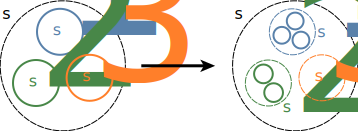
\includegraphics[width=0.7\linewidth]{sharding-meaning}
  \caption{Sharding of OR-Sets}
  \label{fig:sharding_meaning}
\end{figure}

In order to coordinate incoming requests for each of the replicated set, a
client entity should be used to forward the usual $\textit{add}(e)$,
$\textit{remove}(e)$, and $\textit{lookup}(e)$ operations to the corresponding
subset. For this purpose, the client can employ any partitioning function, such
as a hash function with uniform distribution, which maps each element $e$ to a
shard. The client is also responsible for initiating the \textit{merge}
operation between two clusters to pull the updates from all shards in the remote
cluster and distribute them according to the same hash function to the shards in
the local cluster.

\begin{algorithm}[t]
\small{
	\floatname{algorithm}{Specification}
	\caption{SOR-Set with delta-based synchronization}
 	\label{alg:sor_set}                       

 	\begin{algorithmic}[1]
      \State \Payload $A_{i}^{j} = \varnothing, R_{i}^{j} = \varnothing, T_{i}^{j} = [\,][\,], \forall j \in \{1,\ldots,|rc_{i}|\}$
      \State \textcolor{gray}{\Comment{$rc_{i}$ - Replica cluster $i$; $rs_{i}^{j}$ - Replica shard $j$ of $rc_{i}$}}

 	  \State \Query $lookup_{i}(e) : \text{boolean}$
 	  \State \hspace{\algorithmicindent} \Let $j = hash_{i}(e)$
 	  \State \hspace{\algorithmicindent} \Return $\exists (e, t, rc, rs) \in A_{i}^{j} \land \nexists (e, t, rc, rs, t', rc', rs') \in R_{i}^{j}$

 	  \State \Update $add_{i}(e)$
 	  \State \hspace{\algorithmicindent} \Let $j = hash_{i}(e)$
 	  \State \hspace{\algorithmicindent} \Let $rc = rc_{i}$
 	  \State \hspace{\algorithmicindent} \Let $rs = rs_{i}^{j}$
 	  \State \hspace{\algorithmicindent} \Let $t = T_{i}^{j}[rc][rs] + 1$
 	  \State \hspace{\algorithmicindent} $A_{i}^{j} \coloneqq A_{i}^{j} \cup \{(e, t, rc, rs)\}$
 	  \State \hspace{\algorithmicindent} $T_{i}^{j}[rc][rs] \coloneqq t$

 	  \State \Update $remove_{i}(e)$
 	  \State \hspace{\algorithmicindent} \Pre $lookup_{i}(e)$
 	  \State \hspace{\algorithmicindent} \Let $j = hash_{i}(e)$
 	  \State \hspace{\algorithmicindent} \Let $rc' = rc_{i}$
 	  \State \hspace{\algorithmicindent} \Let $rs' = rs_{i}^{j}$
 	  \State \hspace{\algorithmicindent} \Let $t' = T_{i}^{j}[rc'][rs'] + 1$
 	  \State \hspace{\algorithmicindent} $R_{i}^{j} \coloneqq R_{i}^{j} \cup \{(e, t, rc, rs, t', rc', rs') \mid \exists (e, t, rc, rs) \in A_{i}^{j}\}$
 	  \State \hspace{\algorithmicindent} $T_{i}^{j}[rc'][rs'] \coloneqq t'$
 	  
 	  \State \Compare $(rc_{x}, rc_{y}) : \text{boolean}$
 	  \State \hspace{\algorithmicindent} \Let $\tilde{T}_{x} = version(rc_{x})$
 	  \State \hspace{\algorithmicindent} \Let $\tilde{T}_{y} = version(rc_{y})$
 	  \State \hspace{\algorithmicindent} \Return $(\bigcup_{j} A_{x}^{j} \subseteq \bigcup_{k} A_{y}^{k}) \land (\bigcup_{j} R_{x}^{j} \subseteq \bigcup_{k} R_{y}^{k}) \land (\tilde{T}_{x} \leq \tilde{T}_{y})$
 	  \State \hfill $\forall j \in \{1,\ldots,|rc_{x}|\}; \forall k \in \{1,\ldots,|rc_{y}|\}$
 	  
 	  \State \Merge $(rc_{x}, rc_{y}) : \text{payload}$
 	  \State \hspace{\algorithmicindent} \Let $\tilde{T}_{x} = version(rc_{x})$
 	  \State \hspace{\algorithmicindent} \Let $\tilde{T}_{y} = version(rc_{y})$
 	  \State \hspace{\algorithmicindent} $\forall j \in \{1,\ldots,|rc_{y}|\}$
      \State \hspace{\algorithmicindent} \hspace{\algorithmicindent} \Let $A' = \{(e, t, rc, rs) \in A_{y}^{j} \mid \tilde{T}_{x}[rc][rs] < t\}$
      \State \hspace{\algorithmicindent} \hspace{\algorithmicindent} \Let $R' = \begin{aligned}[t]
                                                                                  & \{(e, t, rc, rs, t', rc', rs') \in R_{y}^{j} \\[-2pt]
                                                                                  & \mid \tilde{T}_{x}[rc'][rs'] < t'\}
                                                                                \end{aligned}$
      \State \hspace{\algorithmicindent} $\forall j \in \{1,\ldots,|rc_{x}|\}$
      \State \hspace{\algorithmicindent} \hspace{\algorithmicindent} \Let $Z.A_{x}^{j} = A_{x}^{j} \cup \{(e, t, rc, rs) \in A' \mid j = hash_{x}(e)\}$
      \State \hspace{\algorithmicindent} \hspace{\algorithmicindent} \Let $Z.R_{x}^{j} = \begin{aligned}[t]
                                                                                          & R_{x}^{j} \cup \{(e, t, rc, rs, t', rc', rs') \in R' \\[-2pt]
                                                                                          & \mid j = hash_{x}(e)\}
                                                                                         \end{aligned}$
      \State \hspace{\algorithmicindent} \hspace{\algorithmicindent} \Let $Z.T_{x}^{j} = max(T_{x}^{j}, \tilde{T}_{y})$
      \State \hspace{\algorithmicindent} \Return $Z$
	\end{algorithmic}
 }
\end{algorithm}

Specification~\ref{alg:sor_set} synthesizes the usual state-based operations.
Each replica $i$ of the set is stored in a \textit{replica cluster} $rc_{i}$.
Inside the cluster $rc_{i}$, the set is partitioned into $|rc_{i}|$ subsets,
called \textit{replica shard}s $rs_{i}^{j}$. Therefore, any shard is uniquely
identified by the pair of identifiers $(rc, rs)$. Based on this observation,
instead of using a timestamp vector to keep track of the latest versions for the
replicas as in the previous section, a vector of timestamp vectors $T$ is
used. $T$ has as many components as there are clusters, while $T[rc_{i}]$ has
$|rc_{i}|$ components, one for each shard. Like before, each cell $T[rc][rs]$
stores the latest version of the logical clock of the shard $(rc, rs)$. Each
shard has its own $T$. Since when adding or removing an element from the source
replica, it will be added or, respectively, removed from only one shard $(rc,
rs)$, i.e. the one computed by the hash function, each update can be uniquely
tagged with the tuple $(t, rc, rs)$, where $t$ is the timestamp generated at
$(rc, rs)$.

Returning to the specification, the payload is also distributed: $A_{i}^{j}$,
$R_{i}^{j}$, and $T_{i}^{j}$ are, respectively, the set of added and removed
elements and the vector of timestamps for shard $rs_{i}^{j}$. The set operations
follow the same principle as before. Merging the state of a remote replica from
cluster $rc_{y}$ into the local state in cluster $rc_{x}$ is also similar. We
just need to compute a minimum version $\tilde{T}_{x}$ first for the whole
cluster by combining the information from all $T_{x}^{j}$ using
$version(rc_{x})$ defined as:
% \small
\begin{align*}
\tilde{T}_{x}[rc][rs] = \begin{cases}
                            max (\bigcup_{j \in \{1,\ldots,|rc_{x}|\}} T_{x}^{j}[rc][rs]) & \text{if } rc = rc_{x}, \\
                            min (\bigcup_{j \in \{1,\ldots,|rc_{x}|\}} T_{x}^{j}[rc][rs]) & \text{otherwise}
                        \end{cases}
\\
\hfill \forall rc = rc_{i}, i \in \{1,\ldots,N\}; \forall rs = rs_{i}^{j}, j \in \{1,\ldots,|rc_{i}|\}.
\end{align*}
% \normalsize

We set the minimum from all $T_{x}^{j}$ component-wise, except for
$\tilde{T}_{x}[rc_{x}]$, where we choose the maximum instead since each shard in
$rc_{x}$ increments its own counter only. We do the same for cluster $rc_{y}$.

Some important observations are worth mentioning. First, the \textit{merge}
operation remains unobtrusive like for all CRDTs: clients can issue requests to
the set while the operation progresses in the background. Since the minimum
version $\tilde{T}_{y}$ is computed first, the remote cluster $rc_{y}$ can
meanwhile process any subsequent updates. They will be pulled with the next
merge. Analogously, because at the end each $T_{x}^{j}$ is updated to the
maximum between the current one and the remote one component-wise, the local
cluster can in this time process any incoming client requests. Therefore, both
sets can be updated while the synchronization takes place. 

Second, this algorithm is resilient to shard failures in both local and remote
clusters. An unreachable shard in the local cluster leads to a potential bigger
$\tilde{T}_{x}$ except for $\tilde{T}_{x}[rc_{x}]$. This means that not all
updates will be fetched. As soon as the failed shard restores, its lagging
timestamp will lead to a smaller $\tilde{T}_{x}$ and the next merge will thus
include the missing updates plus some of the already fetched ones. For the
remote cluster, an unreachable shard has the same consequence: $T_{x}^{j}
\coloneqq max(T_{x}^{j}, \tilde{T}_{y})$ will set smaller values in
$T_{x}^{j}[rc_{y}]$ and missed updates will be fetched with the next merge after
the shard restores. Optionally, a master-slave replication scheme can be used to
ensure fault-tolerance for any shard.

\begin{proof}[Proof that sharding maintains the CRDT properties]
Consider a replica state as $s_{i} = (A_{i}, R_{i}, \tilde{T}_{i})$, where
$A_{i} = \bigcup_{j \in \{1,\ldots,|rc_{i}|\}} A_{i}^{j}$ and $R_{i} =
\bigcup_{j \in \{1,\ldots,|rc_{i}|\}} R_{i}^{j}$. Thus, a set is characterized
by the contributions of all its subsets. The partial order is then $(S,
\sqsubseteq)$, $\forall s_{i} \in S$ and $\sqsubseteq$ given by \textit{compare}
method. Update operations \textit{add} and \textit{remove} advance the state in
the partial order as they both add elements to the set and increase $\tilde{T}$.
\textit{Merge} computes the set union between $A_{x}$ and $A_{y}$ and between
$R_{x}$ and $R_{y}$, respectively. Also, because each $T_{x}^{j}$ is updated
with the maximum between $T_{x}^{j}$ and $\tilde{T}_{y}$, the newly obtained
$\tilde{T}_{x}$ will be the maximum between $\tilde{T}_{x}$ and $\tilde{T}_{y}$.
Therefore \textit{merge} computes the LUB.
\end{proof}

\section{Garbage Collection}
\label{sec:garbage_collection}

\section{Comparison with Previous Work}
\label{sec:previous_work}

The fundamental principles on database replication are laid out
in~\cite{lindsay} and a number of techniques are discussed there to achieve
consistency. The traditional \textit{strong consistency} approach imposes a
global total order on updates to serialize
them~\cite{Lamport:1978:TCO:359545.359563}. This conflicts with availability and
partition-tolerance~\cite{Gilbert:2002:BCF:564585.564601} and leads to
performance and scalability bottlenecks. \textit{Sequential consistency} is
another model, weaker than strong consistency, but undecidable in
practice~\cite{Qadeer:2003:VSC:939835.940001}. A survey on other models is
presented in~\cite{Mosberger:1993:MCM:160551.160553}.

Techniques for achieving eventual consistency for large-scale distributed
systems have been an active focus point in recent research. This is mostly due
to the explosion of Internet-based and peer-to-peer services. However, the
origins of the principles behind CRDTs can be found in the apparent unrelated
area of file systems. The state-based approach was introduced for register-like
objects, where the only operation is assignment. It is widely used in
NFS~\cite{Sandberg85designand} and AFS~\cite{Howard:1988:SPD:35037.35059} file
systems and in key-value stores such as Amazon's
Dynamo~\cite{DeCandia:2007:DAH:1294261.1294281}. The mathematical foundations
were laid by Baquero and Moura~\cite{scadt4} and later extended by Shapiro and
Pregui\c{c}a in their work on Treedoc~\cite{Preguica:2009:CRD:1584339.1584604}
in order to support the operation-based approach, thus coining the term of CRDT.
Examples of implementations for this second approach are found in Bayou's
anti-entropy protocol~\cite{Petersen:1997:FUP:268998.266711} and the IceCube
cooperative system~\cite{preguica:inria-00445758}. Later, a formal definition
and rigorous system model for CRDT were published in
\cite{shapiro:inria-00555588} and \cite{Shapiro:2011:CRD:2050613.2050642}.
These are the first works to engage a comprehensive and systematic study on
CRDTs.

Several designs of replicated sets have been proposed, but many of them present
anomalies. Amazon's Dynamo shopping
cart~\cite{DeCandia:2007:DAH:1294261.1294281} uses registers in its
implementation. It takes the union of concurrent assignments, multiple values
are later reduced to a single one. The problem is that a removed element can
reappear. In a 2P-Set~\cite{Wuu:1984:ESR:800222.806750}, adding an element after
it has been removed has not effect. Furthermore, this design imposes
synchronization for reclaiming the tombstones. In
Section~\ref{sec:existing_sets} we gave more examples for replicated sets and
concluded that the OR-Set behaves intuitively.


\section{Conclusions}
\label{sec:conclusions}

Achieving consistency in large-scale distributed systems is not an easy task. To
make things more difficult, designers need to also ensure high-throughput,
low-latencies accesses to the databases. However, building reliable distributed
systems demands trade-offs between consistency and availability as stated by the
CAP theorem~\cite{Gilbert:2002:BCF:564585.564601}. Eventual consistency is a
technique of compromise, widely adopted, but lacking a rigorous theoretical
foundation which makes current approaches ad-hoc and
error-prone~\cite{DeCandia:2007:DAH:1294261.1294281}.

The concept of CRDTs defines replicated data types that have mathematical
properties conferring them a form of eventual consistency, strong eventual
consistency. This model can be described from two equivalent perspectives:
a) state-based: object replicas apply updates locally and later exchange and
merge their states, and b) operation-based: update operations are distributed
among replicas over a reliable broadcast communication channel. Both approaches
guarantee convergence towards a common state without application-level conflict
resolutions, roll-backs, or consensus among
replicas~\cite{Terry:1995:MUC:224056.224070}. Because this model imposes strong
constraints on the type specification, it is not universal though.

In this paper we focused on designs for conflict-free replicated sets and gave
number of practical examples. We introduced two improvements to the original
OR-Set specification: an algorithm for efficient delta-based synchronization and
an extension for replica sharding. Lastly, we proposed a garbage collection
mechanism to support lifetime-limited elements and to alleviate the problem of
unbounded database growth. On the practical side, to the authors' knowledge,
this is the first implementation of a CRDT in the sense of the system model
described in this chapter. Proof-of-concept examples exists~\cite{ericmoritz,
dominictarr}, but they focus only on testing the specifications for CRDTs
locally and in-memory, without a real database store support.

Based on this type, more complex structures can be built. Maps can be
implemented as sets of registers and graphs can include two sets: one for
vertices and another for edges.


\bibliographystyle{IEEEtran}
\bibliography{refs}

\end{document}
